\section{Initial design considerations}
The first thing we decided was the number of actuators.
Most of segway robots include two motors for the motion control, but
we added a third on in order to control the inclination.
So we ended up with three motors in total because we want to control
three degrees of freedom (inclination and speed of both wheels).

In order to control the inclination of the platform we needed to produce
an external torque to the platform. We considered three methods: accelerating
a flywheel, holding a pendulum in a non-vertical position and air friction
with a fan. We discarded the last one due to the high speeds we needed to obtain
a reasonable torque on the platform.

Both methods have strengths in different situations, so we decided to build a mixed
piece that could combine both. The flywheel mode allows to deliver the maximum torque from
the beginning but fails to deliver a continuous torque due to the motor achieving max speed.
In the other hand the pendulum allows the system to apply a constant amount of torque over time.

We took two more restriction in our design. The first one symmetry along the motors/inclination
axis in order to have an equilibrium in all possible inclinations without the need of external forces.
We also took in consideration that some experiments may start produce arbitrary rotations of the platform,
so none of the configurations should touch the ground to avoid crashes. Figure \ref{fig:Side render view} illustrates this last restriction.

The design of the robot was done with the 3D design software \href{https://www.freecadweb.org/}{Free-cad} and 
most of the parts were 3D printed. 3D printing has also its own restrictions, for example not being able to print
parts bigger than 25 cm. All part files are uploaded to the GitHub repository \url{https://github.com/tarragoesteve/TFM}
under the hardware folder. So anyone can build this robot.

You can see the main views of an initial design on Figure \ref{fig:Isometric render view},
\ref{fig:Front render view}, \ref{fig:Top render view} and \ref{fig:Side render view}.

\begin{figure}
	\centering
	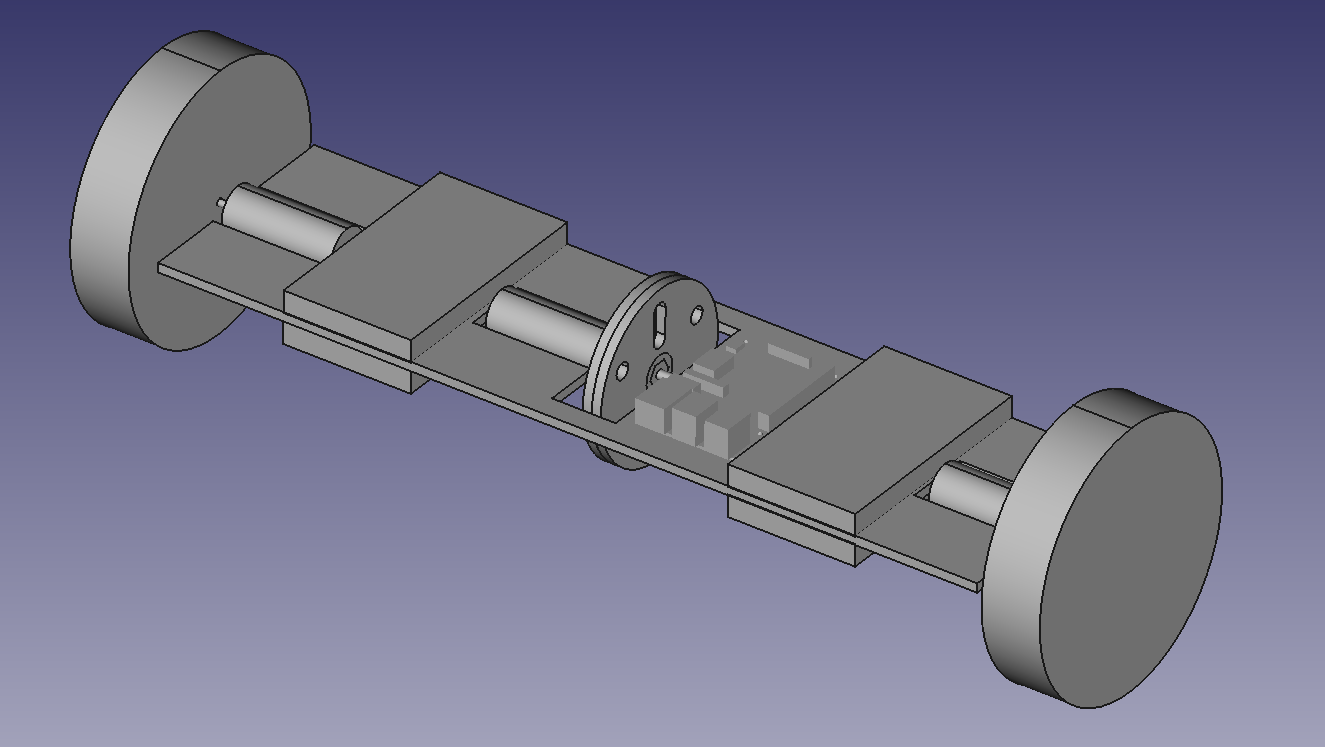
\includegraphics[width=10cm]{img/isometric_view.png}
	\caption{Isometric render view}
	\label{fig:Isometric render view}
\end{figure}
\begin{figure}
	\centering
	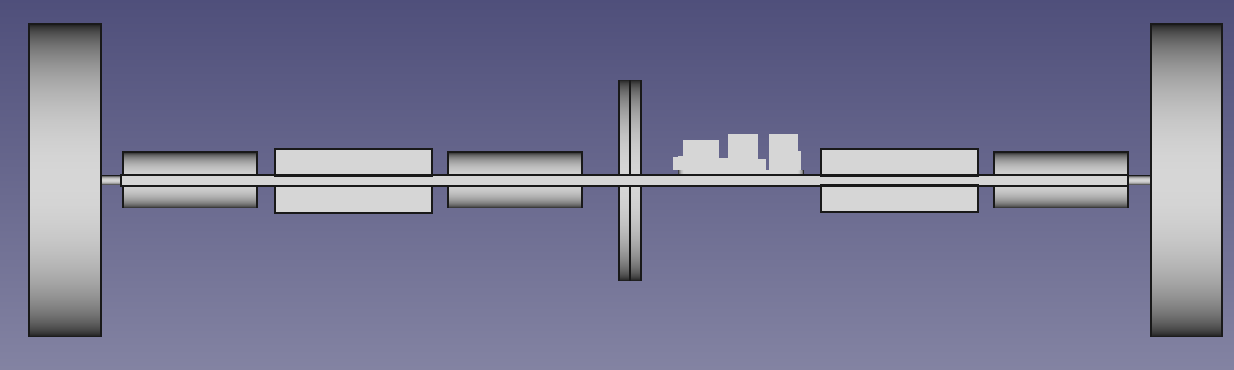
\includegraphics[width=10cm]{img/front_view.png}
	\caption{Front render view}
	\label{fig:Front render view}
\end{figure}
\begin{figure}
	\centering
	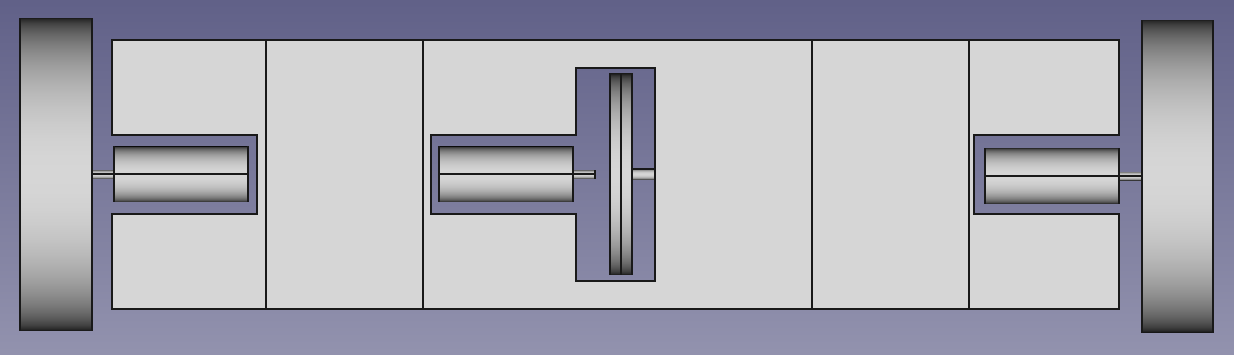
\includegraphics[width=10cm]{img/top_view.png}
	\caption{Top render view.}
	\label{fig:Top render view}
\end{figure}
\begin{figure}
	\centering
	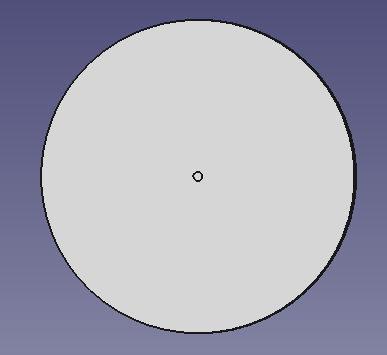
\includegraphics[width=4cm]{img/side_view.png}
	\caption{Side render view.}
	\label{fig:Side render view}
\end{figure}

\subsection{Flywheel design} \label{sec: flywheel design}
\begin{figure}
	\centering
	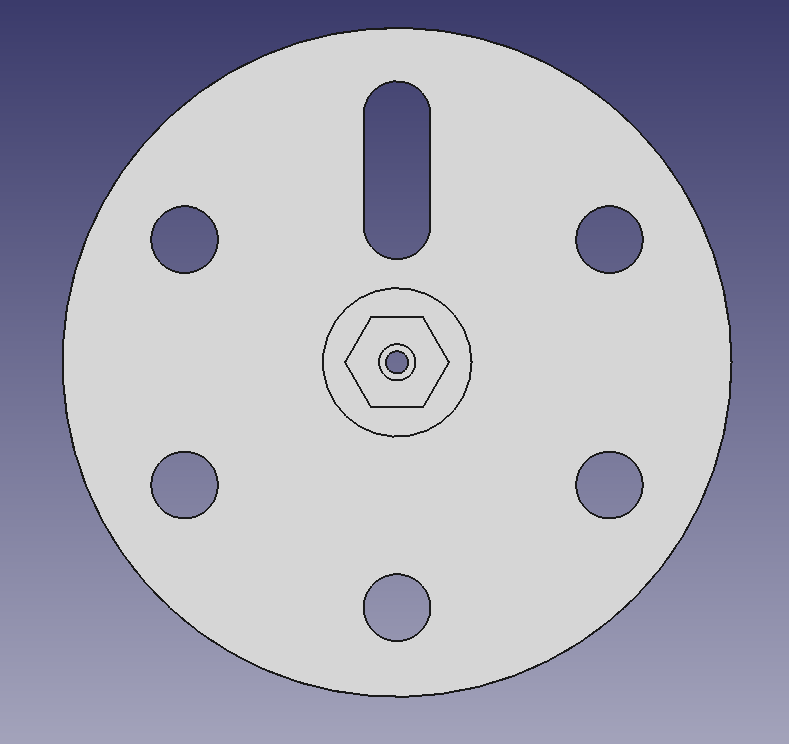
\includegraphics[width=5cm]{img/fly_wheel_side.png}
	\caption{Flywheel side render view.}
	\label{fig:Fly wheel side render view}
\end{figure}

To control the inclination of the body two strategies are taken into account.
Creating torque by a pendulum or accelerating the flywheel.
In order to experiment with both of them we designed a part to allow
both configurations by placing weights in different spots, see figure
\ref{fig:Fly wheel side render view}.

In order to create a configuration with maximum pendulum torque
we have done the following computation. We denote the pendulum
torque by $\tau$, consider the masses are cylinders of mass $m_{cylinder}$
with radius $r_{cylinder}$ and width $w$ and the radius of the flywheel is $r_{flywheel}$.
We want to place all $N$ masses at the same distance of the center of the flywheel ($r_{max}$) in
a regular polygon except for one mass that will be at $r_{min}$. See figure \ref{fig:Fly wheel side render view}.

Each mass weights:
\[ m_{cylinder} = \rho \cdot w \cdot \pi \cdot r_{cylinder}^2 \]

We neglect the mass of the flywheel structure versus the mass of the cylinders. All
the gravitational torque is created by the cylinder masses and all of them are compensated
with the opposite weight except for the two masses with different radius.

One of the weights can be placed along a track. The distance to the center will
vary from $r_{min} = r_{cylinder} + r_{motor-axis} \approx r_{cylinder} $ to $r_{max} = r_{flywheel} - r_{cylinder}$.

The maximum torque takes place when these two masses are aligned horizontal with respect to the ground and the movable weight is at distance $r_{min}$ from the center.

\[ \tau _{max} (r_{cylinder}) =  m_{cylinder} \cdot g \cdot r_{max} -  m_{cylinder} \cdot g \cdot r_{min} =
	m_{cylinder}\cdot g \cdot (r_{flywheel} - 2 \cdot r_{cylinder}) \]

In order find the radius $r_c$ that maximizes $\tau$ we first compute the derivative:
\[\frac{\partial \tau _{max} (r_{cylinder})}{\partial r_c} = g \cdot(\frac{\partial m}{\partial r_c} \cdot (r_f - 2 \cdot r_c) -  m_{cylinder} \cdot 2)\]

\[ \frac{\partial  m_{cylinder}}{\partial r_{cylinder}} = 2 \cdot \rho \cdot w \cdot \pi \cdot  r_{cylinder}\]

And make it zero to find the maximum:

\[\frac{\partial \tau _{max} (r_{cylinder})}{\partial r_{cylinder}} = 0\]

Substituting and simplifying we get:

\[\frac{\partial m}{\partial r_{cylinder}} \cdot (r_{flywheel} - 2 \cdot r_{cylinder}) =
	m_{cylinder} \cdot 2 \Rightarrow 2 \cdot \rho \cdot w \cdot \pi \cdot  r_{cylinder}\ \cdot (r_{flywheel} - 2 \cdot r_{cylinder}) = \rho \cdot w \cdot \pi \cdot r_c^2 \cdot 2 \]

\[ \Rightarrow r_c\ \cdot (r_{flywheel} - 2 \cdot r_{cylinder}) =  r_{cylinder}^2
	\Rightarrow (r_{flywheel} - 2 \cdot r_{cylinder}) =  r_{cylinder}
	\Rightarrow \boxed{r_f = 3 \cdot r_{cylinder}}\]


The circumradius $R$ from the center of a regular polygon to one of the vertices is related to the side length $s$ by:

\begin{center}
	\begin{tabular}{ c  c }
		\(\displaystyle R=\frac {s}{2\cdot \sin{\frac {\pi} {n}}} \)
		 &
		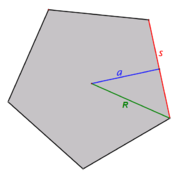
\includegraphics[width=3cm]{img/PolygonParameters.png}
	\end{tabular}
\end{center}

In our case:
\[ R = r_{flywheel} - r_{cylinder}; \]
\[ s = 2 \cdot r_{cylinder}\]

Substituting in the circumradius equation we get n = 6, so we will use up to 6 masses in our flywheel.
We will have a variable number of masses $N$ that we will be able to add to
the flywheel as shown in the following table:
\begin{center}
	\begin{tabular}{c | c | c | c }
		2 & 3 & 4 & 6 \\
		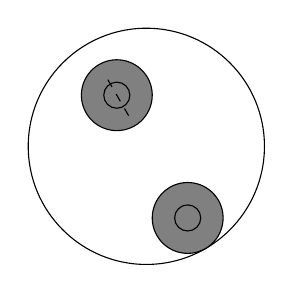
\begin{tikzpicture}[scale=0.5]
			%Circle
			\path node (center) at (0,0) {};
			\draw (center) circle (3);
			%Movable mass
			\draw[rotate=120,fill=gray] (1.5,0) circle (.9) node (moving) [draw,circle]{};
			%Guide
			\draw[dashed,rotate=120] (.9,0) -- (2.1,0);
			%Other masses
			\foreach \i in {2}
				{
					\draw[rotate=60-60*\i,fill=gray] (3-.9,0) circle (.9) node[draw,circle]{};
				}
		\end{tikzpicture}

		  &
		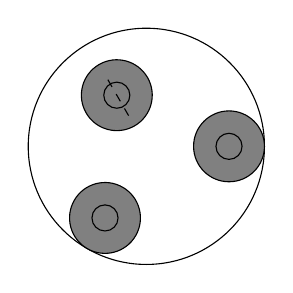
\begin{tikzpicture}[scale=0.5]
			%Circle
			\path node (center) at (0,0) {};
			\draw (center) circle (3);
			%Movable mass
			\draw[rotate=120,fill=gray] (1.5,0) circle (.9) node (moving) [draw,circle]{};
			%Guide
			\draw[dashed,rotate=120] (.9,0) -- (2.1,0);
			%Other masses
			\foreach \i in {1,3}
				{
					\draw[rotate=60-60*\i,fill=gray] (3-.9,0) circle (.9) node[draw,circle]{};
				}
		\end{tikzpicture}
		  &
		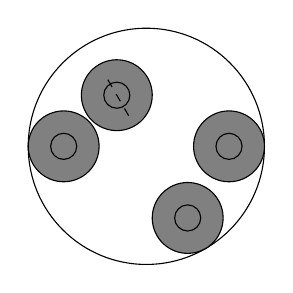
\begin{tikzpicture}[scale=0.5]
			%Circle
			\path node (center) at (0,0) {};
			\draw (center) circle (3);
			%Movable mass
			\draw[rotate=120,fill=gray] (1.5,0) circle (.9) node (moving) [draw,circle]{};
			%Guide
			\draw[dashed,rotate=120] (.9,0) -- (2.1,0);
			%Other masses
			\foreach \i in {1,2,4}
				{
					\draw[rotate=60-60*\i,fill=gray] (3-.9,0) circle (.9) node[draw,circle]{};
				}
		\end{tikzpicture}
		  &

		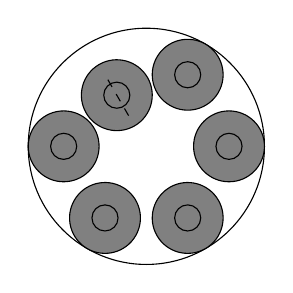
\begin{tikzpicture}[scale=0.5]
			%Circle
			\path node (center) at (0,0) {};
			\draw (center) circle (3);
			%Movable mass
			\draw[rotate=120,fill=gray] (1.5,0) circle (.9) node (moving) [draw,circle]{};
			%Guide
			\draw[dashed,rotate=120] (.9,0) -- (2.1,0);
			%Other masses
			\foreach \i in {1,2,3,4,6}
				{
					\draw[rotate=60-60*\i,fill=gray] (3-.9,0) circle (.9) node[draw,circle]{};
				}
		\end{tikzpicture}
		\\
	\end{tabular}
\end{center}
